\documentclass{../../../ksp}

\usepackage{graphicx}
\graphicspath{ {./} }

\title{KSP 35--3--3}
\author{Daniel Culliver}
\date{Únor 2023}

\begin{document}

\maketitle

\section*{Řešení}

Nejprve začnu uvedením ukázkového stromu, jaký bychom mohli dostat na vstupu.

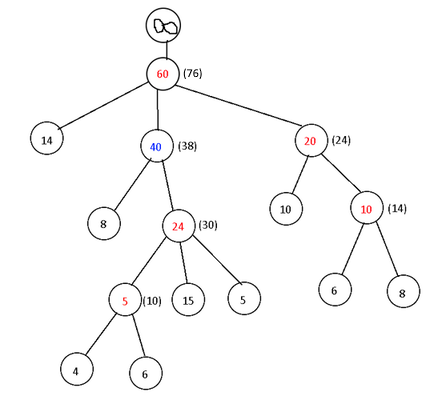
\includegraphics{strom2}

Černými čísly jsou značeny reálný příkon na prodlužovačce či zařízení.
Barevnými čísly jsou značeny maximální příkon prodlužovaček, červené jsou přetížené, modré jsou v pořádku.

Můžeme si všimnout, že i přes to, že jsou 5 z prodlužovaček přetížené, při odstranění 6 a 8 v nejspodnějších vrstvách stromu
nakonec bude přetížený jen nejvrchnější. Poté tedy stačí jen odebrat libovolné zařízení, aby se úloha splnila.

Toto nám ale napovídá, že je lepší vyřešit prodlužovačky na spodních vrstvách a až poté jít nahoru.
Tedy, náš algoritmus bude využívat DFS.\@

Základ našeho algoritmu je velmi jednoduchý. Pro každou prodlužovačku potřebujeme vědět všechna zařízení do které vede
a ideálně i který z nich je největší. Proto bude každá prodlužovačka mít haldu všech zařízení do kterých vede, s největším na vrcholu.
Toto nám umožní vždy odstranit největší zařízení, když bude prodlužovačka stála přetížená. Můžeme pokaždé odstraňovat největší, protože
my nehledáme nejefektivnější zapojení, jenom funkční zapojení, kde jediná podmínka je nezatíženost prodlužovaček.

Tedy pro náš ukázkový strom, by náš algoritmus začal přidáním zařízení s příkonem $14$ k nejvrchnější prodlužovačce.
Poté začne prohledávat další prodlužovačku, přidá jí $8$ do haldy a začne prohledávat opět další proluřovašku, která začne také prohledáváním další prodlužovačky.
Tam odstraníme $6$ a protože už není přetížená a už se k ní nevrátíme, můžeme její celou haldu přidat k prodlužovačce, která k ní vede a původní haldu vymažeme.

Při dalším kroku bude mít prodlužovačka s kapacitou $24$ v haldě zařízení $15$, $5$ a $4$.
Tam už nebude potřeba nic odstraňovat, takže opět přidáme všechna tyto zařízení k prodlužovačce nad ní a vymažeme původní haldu.

Takhle bychom prokračovali dál, až bychom pro prodlužovačku vpravo s kapacitou $10$ smazali zařízení s příkonem $8$ a pokračovali bychom dál k vrcholu, který by měl ke konci takovou haldu:

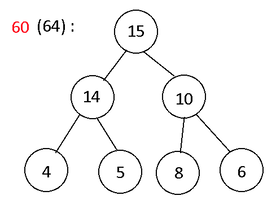
\includegraphics{halda2}

Tady naposledy provedeme krok, kde budeme odstraňovat největší zařízení, dokud prodlužovačka nebude zatížená (v tomhle případě jen jednou)
a tím si ukázali, jak tento algoritmus funguje v praktickém případě.

Samozřejmě, jako výstup musíme udávat počet odstraňených zařízení a i jejich polohu, proto bychom ukládali u každé zařízení i cestu, jak se k němu dostat.
Protože využíváme DFS, toto je naprosto triviální. Pokaždý když narazíme na zařízení, tak jen přidáme krok, kde u něj uložíme cestu k vrcholu, před tím, než ho vložíme do haldy prodlužovačky, do které je zapojený.

Teď spočítáme složitost tohoto řešení a poté ještě uvedeme příklad pseudokódu.

Protože zadaný strom není binární, rozdělíme počet vrcholů na $n$ a $m$, kde $n$ bude počet prodlužovaček (vrcholy s listy) a $m$ počet zařízení (zakončení stromu).
Nejdřív nahlédneme, že DFS projde celkem $n+m$ vrcholů. Každé zařízení přidá do haldy minimálně jednou, a dokonce i více krát, podle toho v jaké hladině se nachází.
Kvůli tomuto kroku je velmi těžké zpočítat komplexitu pro typické příklady, ale jestli nám stačí jen $\BigO$ komplexita, tak můžeme využít takový trik.
Tento trik je velmi jednoduchý, najdeme nejhorší možný strom pro tento algoritmus.

Jak jsme zmínili, každé zařízení vložíme do haldy tolikrát kolik je jejich hloubka, proto bude nejhorší zadání strom, kde každá prodlužovačka vede
jenom k další prodlužovačce, až na poslední, který bude připojený ke všem zařízení. Kdyby nějaké prodlužovačky měli příliš malou kapacitu, tak bychom předem odstranili nějaké zařízení a tím pádem zrychlili algoritmus.
Tudíž, všechny prodlužovačky by měli mít dostatečnou kapacitu až na nejvyšší, který bude mít nulovou kapacitu.

Přesun všech zařízení k nejvyšší prodlužovačce by tedy trvalo $\BigO(n \cdot m \log{m})$. Poslední odstranění zařízení by trvalo jen $\BigO(m\log{m})$,
což vzhledem k předchozí komplexitě zanedbáme.

Prostorová komplexita také není příliš komplikovaná. Prostor všech hald mužeme zanedbat, protože při jejich tvoření můžeme vlastně smazat ty vrcholy, které ji tvořily,
takže prostor vstupu $n+m$ se ve finále zachová a dokonce se i může malinko zlepšit (vymazáním zbytečných vrcholů prodlužovaček). Poslední co nám tedy zbýva spočítat jsou cesty k zařízení, které budou v nich uložené.
Nejhorší případ pro tento výpočet je stejný jako případ o kterém jsme uvažovali pro časovou složitost, tedy každé zařízení by měl cestu o délce $n$.
To v celku vyjde na komplexitu $\BigO(n \cdot m)$. Jinak, v průměrném případě by ta cesta byla nějaký $\log{n}$, ale to se nebere v potaz pro výpočet $\BigO$ komplexity.

Celkově vyjde složitost algoritmu jako $\BigO(n \cdot m \log{m})$ pro časovou a $\BigO(n \cdot m)$ pro prostorovou.

Na konci si ještě uvedeme příklad pseudokódu:

\begin{algorithm*}
    \caption{$specializedDFS(curNode, path)$}
    \begin{algorithmic}
        \Require{node $curNode$, array $path$ of the current path}
            \State{add $curNode$ to the end of $path$}
            \If{$curNode$ has no children} \Comment{$curNode$ is a device}
                \State{$curNode.path \gets path$}
                \State{remove $path.last$ from $path$ \Comment{$path.last$ is now the parent of $curNode$}}
                \State{add $curNode$ to $path.last.heap$ \Comment{Adds the device to the heap of its parent}}
                \State{add $curNode.power$ to $path.last.power$}
                \State{\Return{}}
            \EndIf{}
            \For{every $child$ of $curNode$}
                \State{$specializedDFS(child)$}
            \EndFor{}
            \While{$curNode.capacity$ < $curNode.power$}
                \State{add $curNode.heap.first$ to $result$}
                \State{remove $curNode.heap.first.power$ from $curNode.power$}
                \State{delete $curNode.heap.first$ and reorder the heap}
            \EndWhile{}
            \If{$curNode$ isn't $firstNode$}
                \State{remove $path.last$ from $path$ \Comment{$path.last$ is now the parent of $curNode$}}
                \State{move $curNode.heap$ to $path.last.heap$}
                \State{delete $curNode.heap$ \Comment{You can also just delete the whole node}} 
            \EndIf{}
        \State{\Return{}}
        \Ensure{Array $result$, which contains all removed devices with their paths}
    \end{algorithmic}
\end{algorithm*}

Protože vracíme celý pole, délku toho pole je počet odstraněných zařízení.

\end{document}